\chapter{OpenCL: The Open Source Specification for GPU Programming}

OpenCL stands for Open Computing Language initially proposed by Apple in 2008 and is currently maintained by Khronos Group. The other big companies involved in developing the OpenCL specification include NVIDIA, AMD, Intel etc.

\paragraph{}
OpenCL is a specification i.e. programmers has to write their own implementations which are compliant to the specification. Thus OpenCL is a programming interface which offers a framework to build applications on top of it. This framework allows the user to take the advantage of all the system resources (CPU, GPU, DSP chip etc).

\paragraph{}
OpenCL is designed to support general purpose parallel computation. It can be used for variety of tasks which involves heavy computation and calculation like in computer graphics, digital signal processing, scientific calculations, analysis of financial data and many more.

\section{The OpenCL Architecture}
All work and no play makes Jack a dull boy,All work and no play makes Jack a dull boy,All work and no play makes Jack a dull boy,All work and no play makes Jack a dull boy,All work and no play makes Jack a dull boy...

\subsection{Platform Model}
The platform model consists of a host connected to one or more OpenCL devices. The devices in turn contains compute units (CUs) which is a collection of processing units (PEs) which are responsible for all the computations happening in the device. This is shown in the \textit{figure~\ref{fig:platform_model}}. The developer submits the commands to be executed on the device through the host which is responsible for setting up the device. The device splits up the instructions and data on its processing units to be executed as SIMD or SPMD. 

\begin{figure}[ht]
\centerline{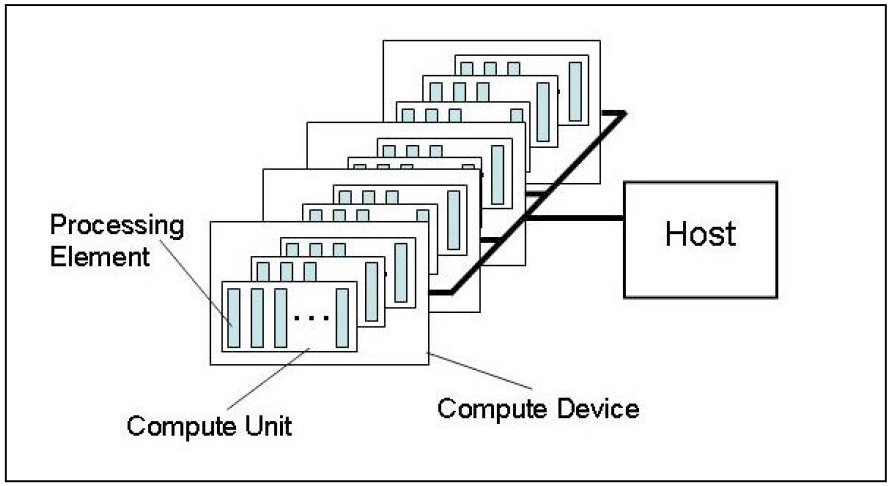
\includegraphics[width=0.7\textwidth]{platform_model.png}}
\caption[Platform Model]%
{\textit{Platform Model ... one host, plus one or more compute devices, each with one or more compute units, each with one or more processing elements \cite[p.~23]{OpenCL_specifications}.} \label{fig:platform_model}}
\end{figure}

\subsection{Execution model}
Programming in OpenCL has two basic parts: the \textbf{host code} that executes on the CPU or the host and the \textbf{kernel codes} that execute on one or more OpenCL device. The way in which the kernel executes on the work units of the device defines the execution model in OpenCL.

\paragraph{}
The basic element of work unit is called \textbf{work-item} which are grouped to form \textbf{work-groups}. All the work-groups are put together to form the \textbf{NDRange} i.e. n-Dimensional Range. The total number of the executable units on the GPU is called the \textbf{global size} which is the size of the NDRange. On the other hand, the size of a work-group is called the \textbf{local size}. It is to be noted that on a GPU, the global size needs to divide evenly into local size.

\paragraph{}
One of the powerful feature of OpenCL, is the natural ability to index the global (i.e. NDRange) and local work space in one, two and three dimensions, using the inbuilt functionality provided by the specification. This concept was well explained in \cite[p.~24-25]{OpenCL_specifications} which is also mentioned below.  

\paragraph{}
For example, consider the 2-dimensional index space in \textit{figure~\ref{fig:execution_model}}. We input the index space for the work-items $(G_{x}, G_{y})$, the size of each work-group $(S_{x}, S_{y})$ and the global ID offset $(F_{x}, F_{y})$. The global indices define an $G_{x}$ by $G_{y}$ index space where the total number of work-items is the product of $G_{x}$ and $G_{y}$. The local indices define a $S_{x}$ by $S_{y}$ index space where the number of work-items in a single work-group is the product of $S_{x}$ and $S_{y}$.  Given the size of each work-group and the total number of work-items we can compute the number of work-groups. A 2-dimensional index space is used to uniquely identify a work-group. Each work-item is identified by its global ID $(g_{x}, g_{y})$ or by the combination of the work-group ID $(w_{x}, w_{y})$, the size of each work-group $(S_{x}, S_{y})$ and the local ID $(s_{x}, s_{y})$ inside the work-group such that 

\begin{equation}
(G_{x}, G_{y}) = (w_{x} \times{S_{x}} + {s_{x}} + {F_{x}},\;\ w_{y} \times{S_{y}} + {s_{y}} + {F_{y}})
\end{equation}

The number of work-groups can be computed as: 
\begin{equation}
(W_{x}, W_{y}) = (G_{x} / S_{x},\;\ G_{y} / S_{y})
\end{equation}

Given a global ID and the work-group size, the work-group ID for a work-item is computed as: 
\begin{equation}
(w_{x}, w_{y}) = ((g_{x} - s_{x} - F_{x}) / S_{x}),\;\ (g_{y} - s_{y} - F_{y}) / S_{y})%
\end{equation}  
  
\begin{figure}[ht]
\centerline{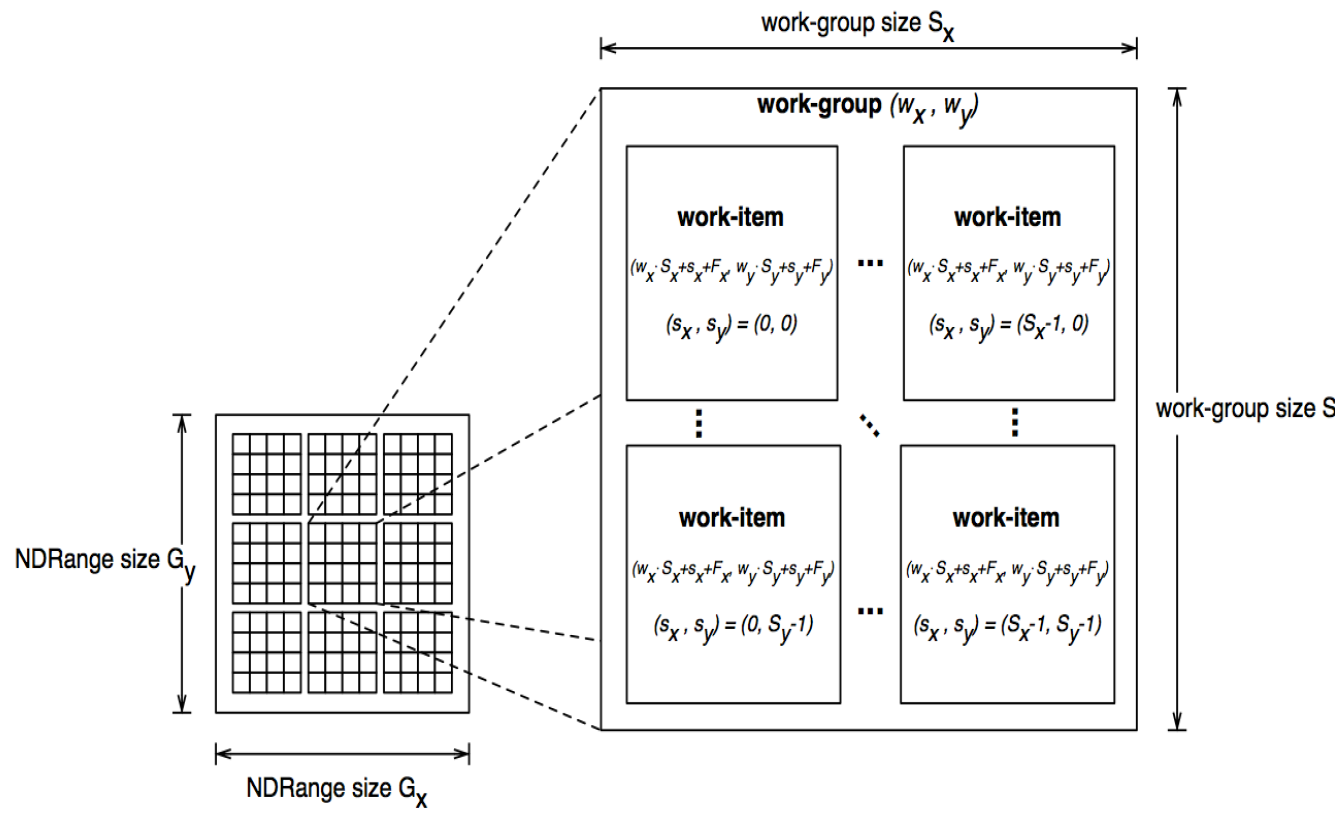
\includegraphics[width=1.0\textwidth]{execution_model.png}}
\caption[Execution model]%
{\textit{An example of NDRange index space showing work-items, their global IDs and their mapping onto the pair of work-groups and local IDs \cite[p.~25]{OpenCL_specifications}.}\label{fig:execution_model}}
\end{figure}

\subsection{Memory Model}
The memory model can be classified into four address spaces which are described in \textit{figure~\ref{fig:memory_model}}. More details on the allocation and usage of the memory available in the device can be found from the \textit{table~\ref{tab:Memory_model}}.
\begin{itemize}
	\item \textbf{\line(90,0){12}global}: It refers to the \textbf{global memory} which allows read and write access to all work-items in the work-group.
	\item \textbf{\line(90,0){12}constant}: It refers to the \textbf{constant memory} which is a part of the global memory. However it remains constant during the execution of the kernel. The initialization and the allocation of the memory objects for the constant memory is done by the host.
	\item \textbf{\line(90,0){12}local}: It refers to the \textbf{local memory} of the work-group which can be shared by all the work-items belonging to that work-group. They are much faster compared to the global memory even though their availability is quite limited.
	\item \textbf{\line(90,0){12}private}: It refers to the \textbf{private memory} of the work-item. Private memory of one work-item is unavailable to other work-items. They act mostly like the resistors and hence are extremely fast.
\end{itemize}

\begin{table*}
	\centering
		\begin{tabular}{| p{1.5cm} | p{2.5cm} | p{2.5cm} | p{2.5cm} | p{2.5cm} |}
			\hline
			 & \textbf{Global} & \textbf{Constant} & \textbf{Local} & \textbf{Private} \\ \hline
			 \textbf{Host} & Dynamic allocation & Dynamic allocation & Dynamic allocation & No allocation \\
			 & & & & \\
			 & Read/Write access & Read/Write access & No access & No access \\ \hline
			 \textbf{Kernel} & No allocation & Static allocation & Static allocation & Static allocation \\
			 & & & & \\
			 & Read/Write access & Read-only access & Read/Write access & Read/Write access \\
			\hline			
		\end{tabular}
	\caption[Memory Region]
	{\textit{Memory Region - Allocation and Memory Access Capabilities \cite[p.~28]{OpenCL_specifications}} \label{tab:Memory_model}}	
\end{table*}

\begin{figure}[ht]
\centerline{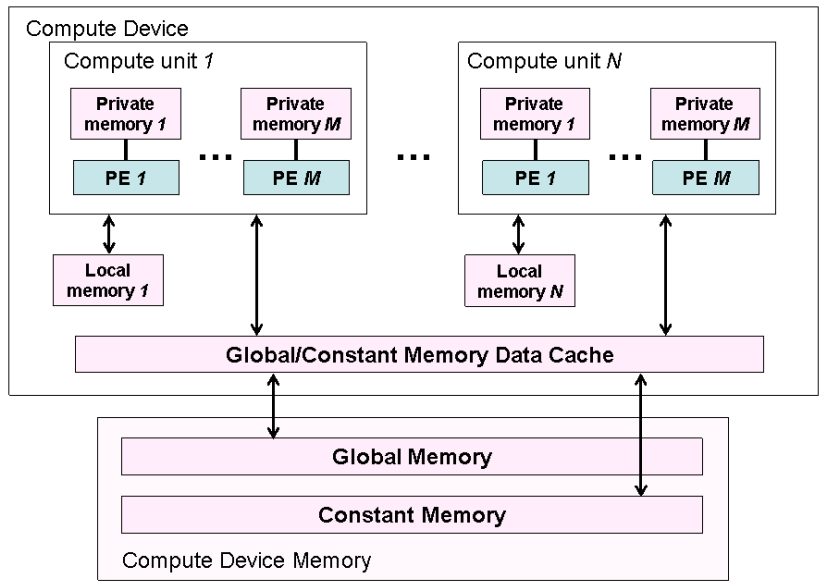
\includegraphics[width=0.7\textwidth]{memory_model.png}}
\caption[Memory model]%
{\textit{Conceptual OpenCL device architecture with processing elements (PE), compute units and devices \cite[p.~28]{OpenCL_specifications}.}\label{fig:memory_model}}
\end{figure}

\subsection{Programming Model}
All work and no play makes Jack a dull boy,All work and no play makes Jack a dull boy,All work and no play makes Jack a dull boy,All work and no play makes Jack a dull boy,All work and no play makes Jack a dull boy...

\subsection{Memory Objects}
All work and no play makes Jack a dull boy,All work and no play makes Jack a dull boy,All work and no play makes Jack a dull boy,All work and no play makes Jack a dull boy,All work and no play makes Jack a dull boy...

\subsection{The OpenCL Framework}
All work and no play makes Jack a dull boy,All work and no play makes Jack a dull boy,All work and no play makes Jack a dull boy,All work and no play makes Jack a dull boy,All work and no play makes Jack a dull boy...

\section{The OpenCL Platform Layer}

\subsection{Querying Platform Info}

\subsection{Querying Devices}

\subsection{Partitioning a Device}

\subsection{Contexts}


\section{The OpenCL Runtime}

\subsection{Command Queues}

\subsection{Buffer Objects}

\subsection{Image Objects}

\subsection{Sampler Objects}

\subsection{Program Objects}

\subsection{Kernel Objects }

\subsection{Executing Kernels}

\subsection{Flush and Finish}


\section{The OpenCL C Programming Language}

\subsection{Supported Data Types}

\subsection{Conversions and Type Casting}

\subsection{Operators}

\subsection{Vector Operations}

\subsection{Address Space Qualifiers}

\subsection{Access Qualifiers}

\subsection{Function Qualifiers}

\subsection{Preprocessor Directive and Macros}


\section{Limitations of OpenCL}


\section{Performance considerations}
How to get the maximum out of the device.

\paragraph{Memory Optimizations}

\paragraph{NDRange Optimizations}

\paragraph{Instruction Optimizations}

\paragraph{Control Flow}